\chapter{Taint Analysis for Member Variables (WORK IN PROGRESS)}
\label{field-tainting}

This chapter describes a concept for adding taint analysis on for member variables of objects to Pixy---the 2007 release of Pixy explicitly mentions this as a ``missing feature''.

\section{Modeling Member Variables as Places for Three-Address Code (TAC)}
\index{member variables}\index{fields}\index{three-address code}

Pixy models variables as ``places'' for three-address code (see section~\ref{tac} on page~\pageref{tac} for details). For taint analysis, it uses this ``place'' abstraction instead of the variables from the parse tree to model the flow of data through the program.

Hence, we need a way to convert access to member variables from the PHP parse tree into TAC places. This needs to happen the \texttt{TacConverter} class which is responsible for the task of creating both the control-flow graph as well as the three-address code from the PHP parse tree.



\subsection{Creating Symbol Table Entries for Objects (READY FOR FEEDBACK)}

\subsubsection{Class Declaration}

For the following code for declaring a class with one field, the corresponding subtree of the PHP parse tree looks like depicted in figure~\ref{fig:parse-tree-foo-class} on page~\pageref{fig:parse-tree-foo-class}.

\begin{phpcode}
class Foo {
  var $field = 42;
}
\end{phpcode}

Note: This piece of code still uses the PHP~4 way of declaring member variables. Using the PHP~5 way with access keywords like \texttt{public}, \texttt{protected} or \texttt{private} would work correspondingly.

\begin{figure}[htb]
  \begin{center}
    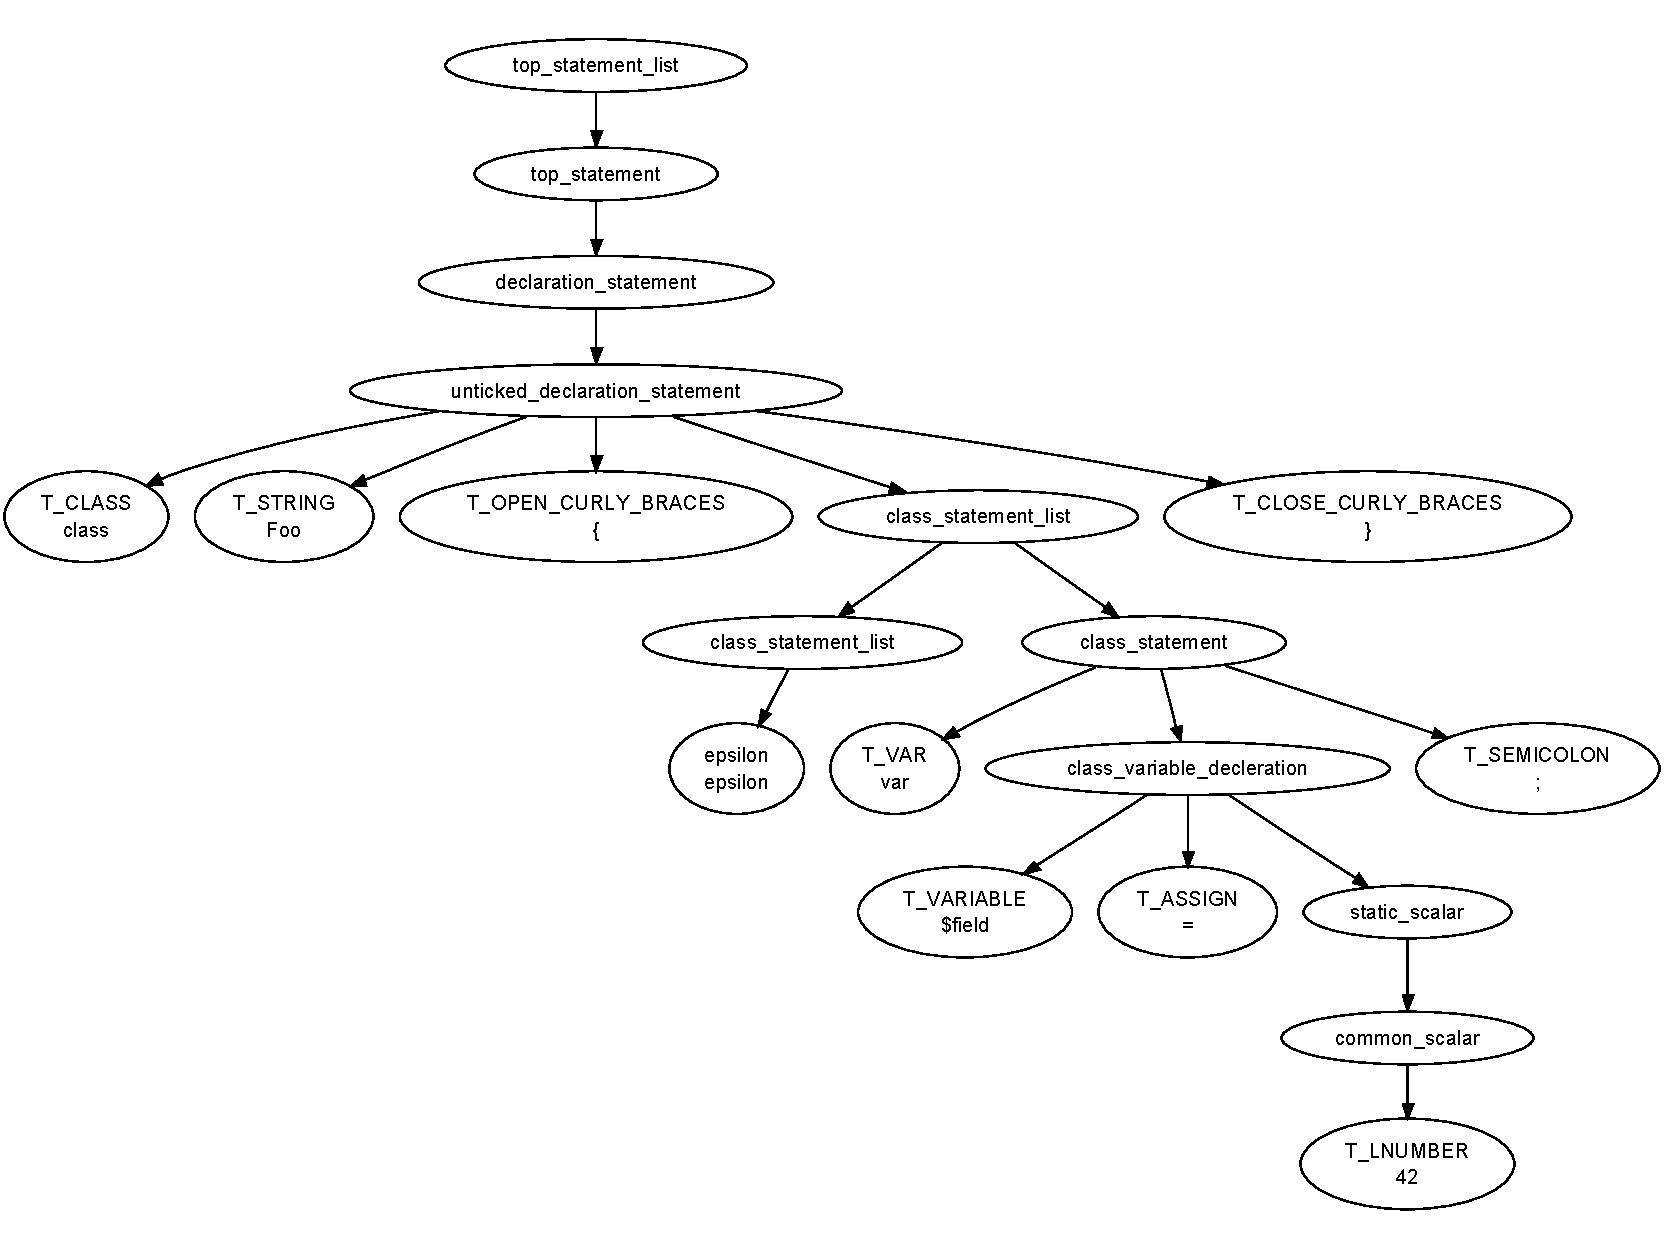
\includegraphics[scale=0.5]{images/parsetree-foo-class-declaration}
   \caption{The subtree of the PHP parse tree for declaring a class \texttt{Foo} with a single field \texttt{\$field} with a default value of \texttt{42}.}
   \label{fig:parse-tree-foo-class}
  \end{center}
\end{figure}

At the point where the \texttt{TacConverter} class encounters the class definition, it would be neither necessary nor helpful to save the taint state of the fields for new class instances: Member variables that have not been written yet by any code can always be considered untainted as the PHP interpreter only allows literals as default values, and Pixy always considers literals to be untainted. Furthermore, uninitialized \emph{member variables} cannot be overwritten using request parameters even if \texttt{register\_globals}\index{register\_globals} is enabled. This is different to the way PHP handles uninitialized local or global variables (see section~\ref{register-globals}).

In addition, the list of declared fields might be only a subset of the fields that are actually accessed in the code: If the PHP interpreter finds a read or write access to an undeclared field, it creates this field for that particular instance on the fly, initializes it with \texttt{null}, and issues a PHP strict warning.


\subsubsection{Class Instantiation}

In the following code example, class declared above gets instantiated in the \texttt{\$foo} variable. The corresponding subtree of the PHP parse tree looks like figure~\ref{fig:parse-tree-new-foo} on page~\pageref{fig:parse-tree-new-foo}.

\begin{phpcode}
$foo = new Foo();
\end{phpcode}

\begin{figure}[htb]
  \begin{center}
    \includegraphics[scale=0.5]{images/parsetree-new-foo}
   \caption{The subtree of the PHP parse tree for creating an instance \texttt{\$foo} of the class \texttt{Foo}.}
   \label{fig:parse-tree-new-foo}
  \end{center}
\end{figure}

Currently, the \texttt{TacConverter} already adds a \texttt{Variable} entry into the current function's symbol table. To closely model the way PHP stores object instances with a separate symbol table per instance (see section~\ref{php-variables} on page~\pageref{php-variables}~ff.), we need a subclass \texttt{ObjectVariable extends Object} that holds a reference to a symbol table instance.

In pseudo-code, processing this assignment would look like this:

\begin{textcode}
AbstractPlace expr_without_variable(subtree) {
  // Extract children from subtree here.

  if (secondChild == T_ASSIGN) {
    assign(subtree);
    return null;
  }

  if (firstChild == T_NEW) {
    return new ObjectVariable();
  }

  // More existing code for processing variables and literals.
}

assign(subTree) {
  variableName = getVariableNameFromLeftSubtree(subtree);
  rightPlace = expr_without_variable(subTree->rightChild->firstChild);
  addVariableToSymbolTable(variableName, rightPlace);
}
\end{textcode}

\paragraph{Note:} In the \texttt{TacConverter} class, the functions are named after the opcodes in the PHP parse tree. The function \texttt{expr\_without\_variable} is called twice because is occurs twice in the subtree (see figure~\ref{fig:parse-tree-new-foo} on page~\pageref{fig:parse-tree-new-foo}).

For the sake of brevity, this pseudo-code omit the part about creating temporary variables if a variable already is present in the symbol table. This feature already is present in Pixy and does not need to be changed.

\subsubsection{Field Access}

To track tainting for member variables, Pixy needs to create ``places'' for all member variables that are accessed---even for those that have not been declared beforehand. (PHP will happily create it on the fly while issuing a PHP warning.)

Both for the left side of assignments as well as for all expressions, we need to add a way to handle field access as places. In addition to the already existing cases (\eg function calls, literals, normal variables etc.), the following cases are new and need to be modeled:

\myTable{
\begin{tabular}{|l|l|l|}
\hline
\bb{case description} & \bb{example} & \bb{parse tree figure} \\
\hline
  simple variable assignment & \texttt{\$x = 42;}  & \ref{fig:simple-variable-assignment} on page~\pageref{fig:simple-variable-assignment} \\
  (already part of Pixy) & & \\
\hline
  one-level field access (left side) & \texttt{\$foo->bar = 42;} & \ref{fig:one-level-field-access-left} on page~\pageref{fig:one-level-field-access-left} \\
\hline
  one-level field access (right side) & \texttt{\$x = \$foo->bar;} & \ref{fig:one-level-field-access-right} on page~\pageref{fig:one-level-field-access-right} \\
\hline
  multi-level field access (left side) & \texttt{\$foo->bar->baz = 42;} & \ref{fig:multi-level-field-access-left} on page~\pageref{fig:multi-level-field-access-left} \\
\hline
  multi-level field access (right side) & \texttt{\$x = \$foo->bar->baz;} & \ref{fig:multi-level-field-access-right} on page~\pageref{fig:multi-level-field-access-right} \\
\hline
  variable field access (left side) & \texttt{\$foo->\$fieldName = 42;} & \ref{fig:variable-field-access-left} on page~\pageref{fig:variable-field-access-left} \\
\hline
  variable field access (right side) & \texttt{\$x = \$foo->\$fieldName;} & \ref{fig:variable-field-access-right} on page~\pageref{fig:variable-field-access-right} \\
\hline
\end{tabular}
}{Field accesses that need to be modeled}{table:field-access-cases}

\paragraph{Note:} Method chaining in PHP is possible, as is field access chaining. After field chaining, method calls are possible. However, even if a method returns an object, chained field accesses on that object are not possible. This approach does not cover method call after field accesses as Pixy already is quite good at finding out which method from which class gets called.


\begin{figure}[htb]
  \begin{center}
    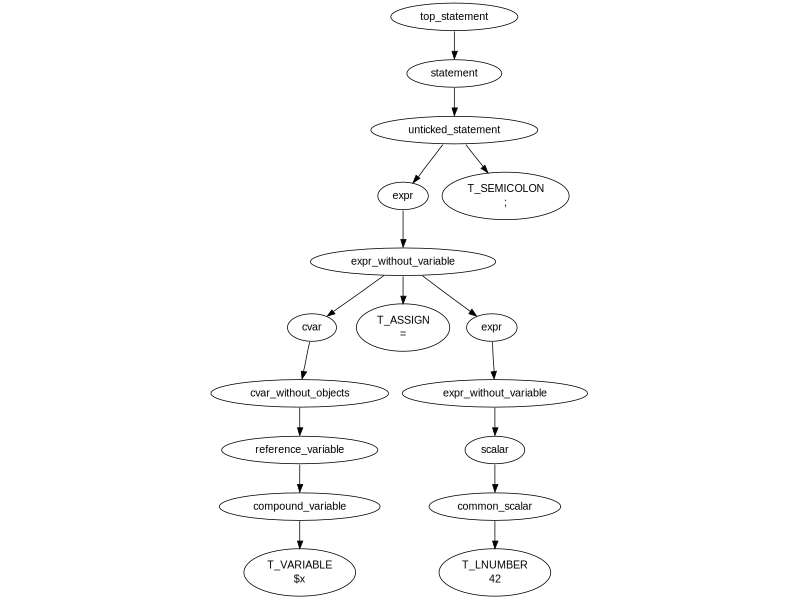
\includegraphics[scale=0.7]{images/simple-variable-assignment}
   \caption{The PHP parse subtree of \texttt{\$x = 42;}.}
   \label{fig:simple-variable-assignment}
  \end{center}
\end{figure}

\begin{figure}[htb]
  \begin{center}
    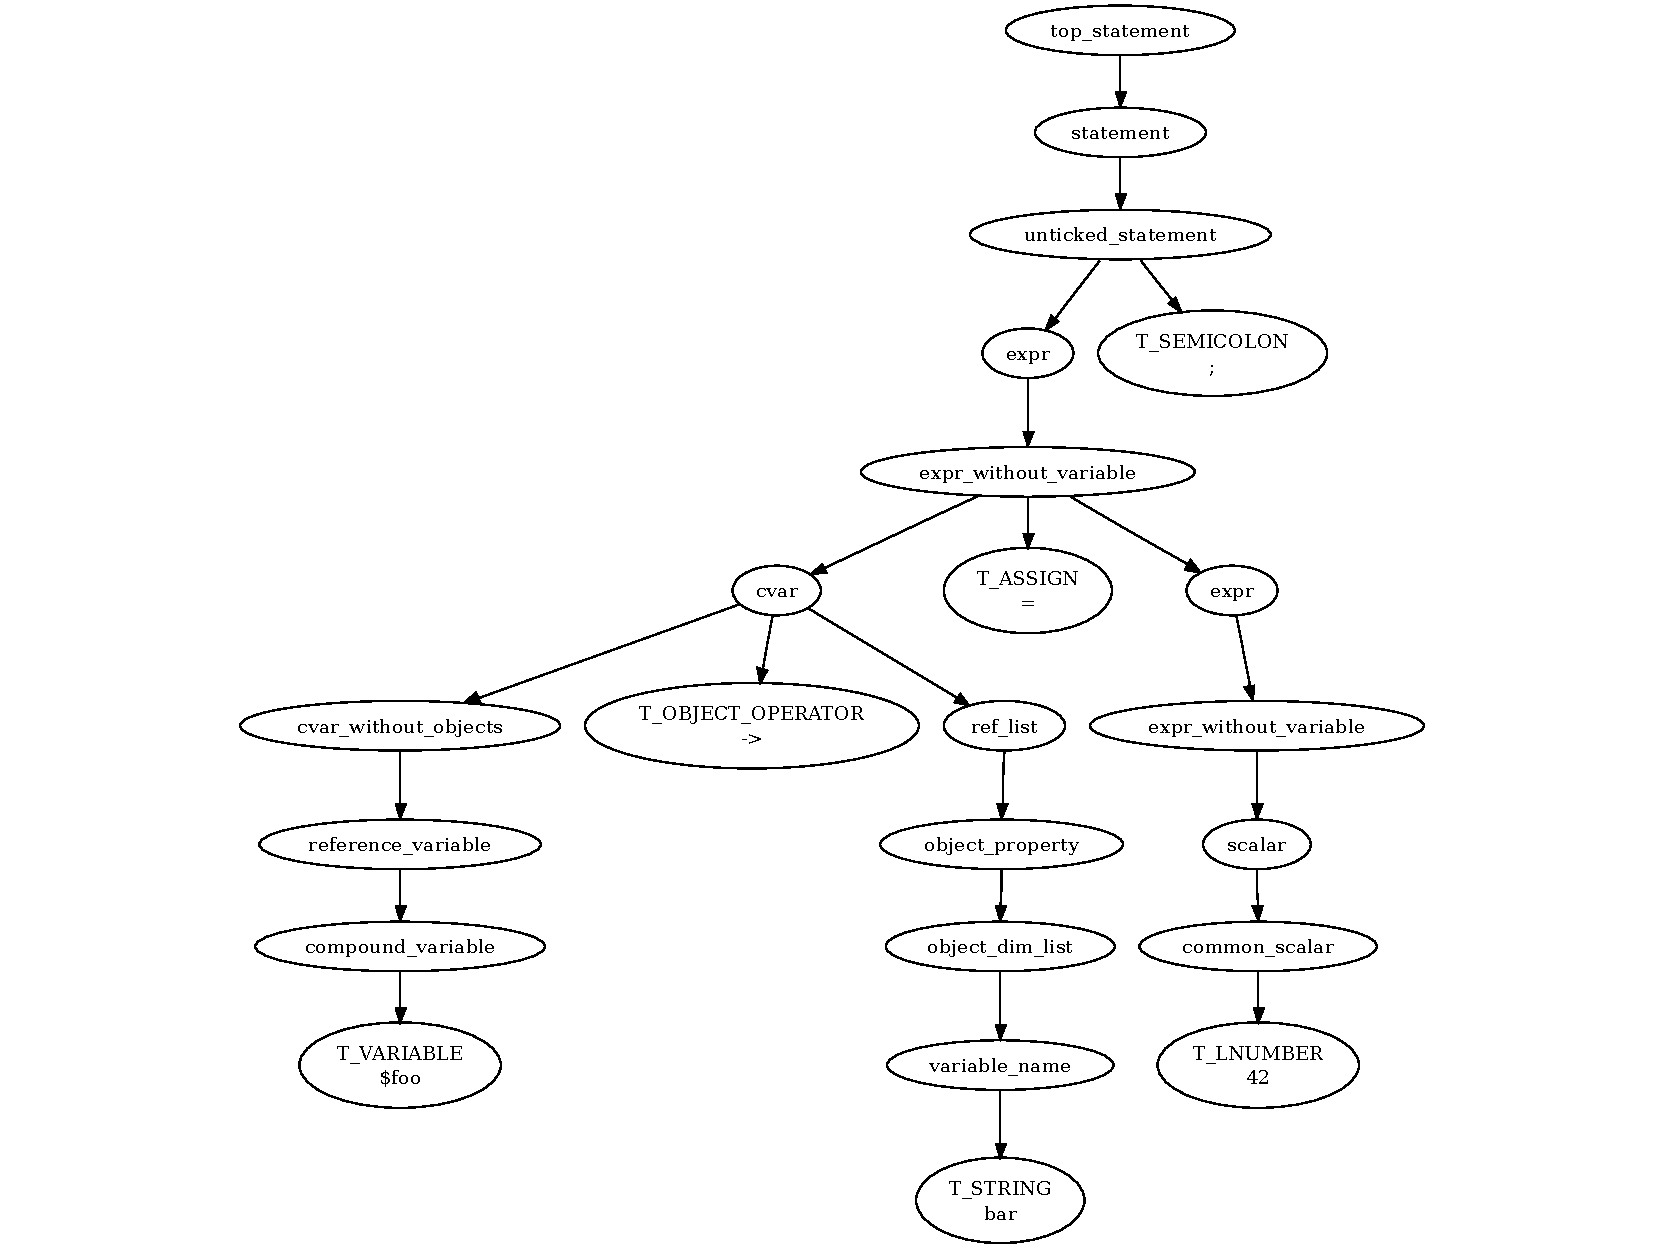
\includegraphics[scale=0.7]{images/one-level-field-access-left}
   \caption{The PHP parse subtree of \texttt{\$foo->bar = 42;}.}
   \label{fig:one-level-field-access-left}
  \end{center}
\end{figure}

\begin{figure}[htb]
  \begin{center}
    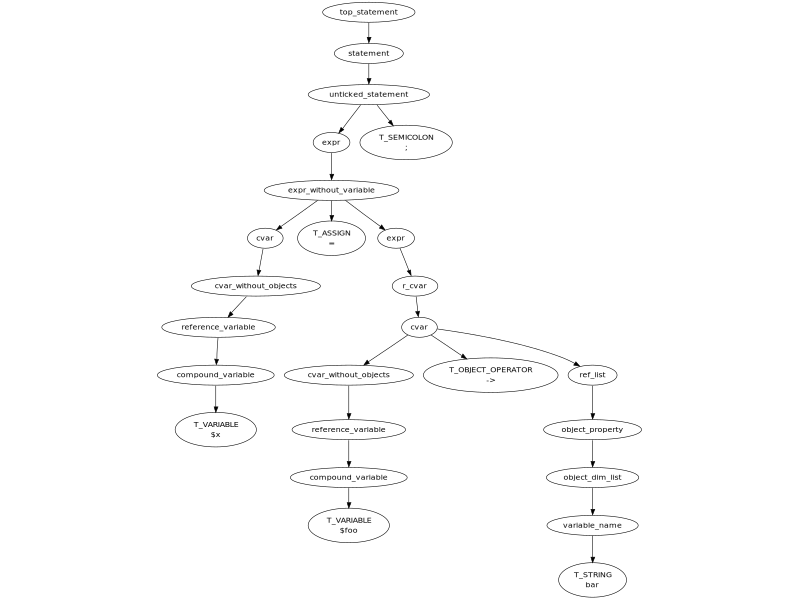
\includegraphics[scale=0.7]{images/one-level-field-access-right}
   \caption{The PHP parse subtree of \texttt{\$x = \$foo->bar;}.}
   \label{fig:one-level-field-access-right}
  \end{center}
\end{figure}

\begin{figure}[htb]
  \begin{center}
    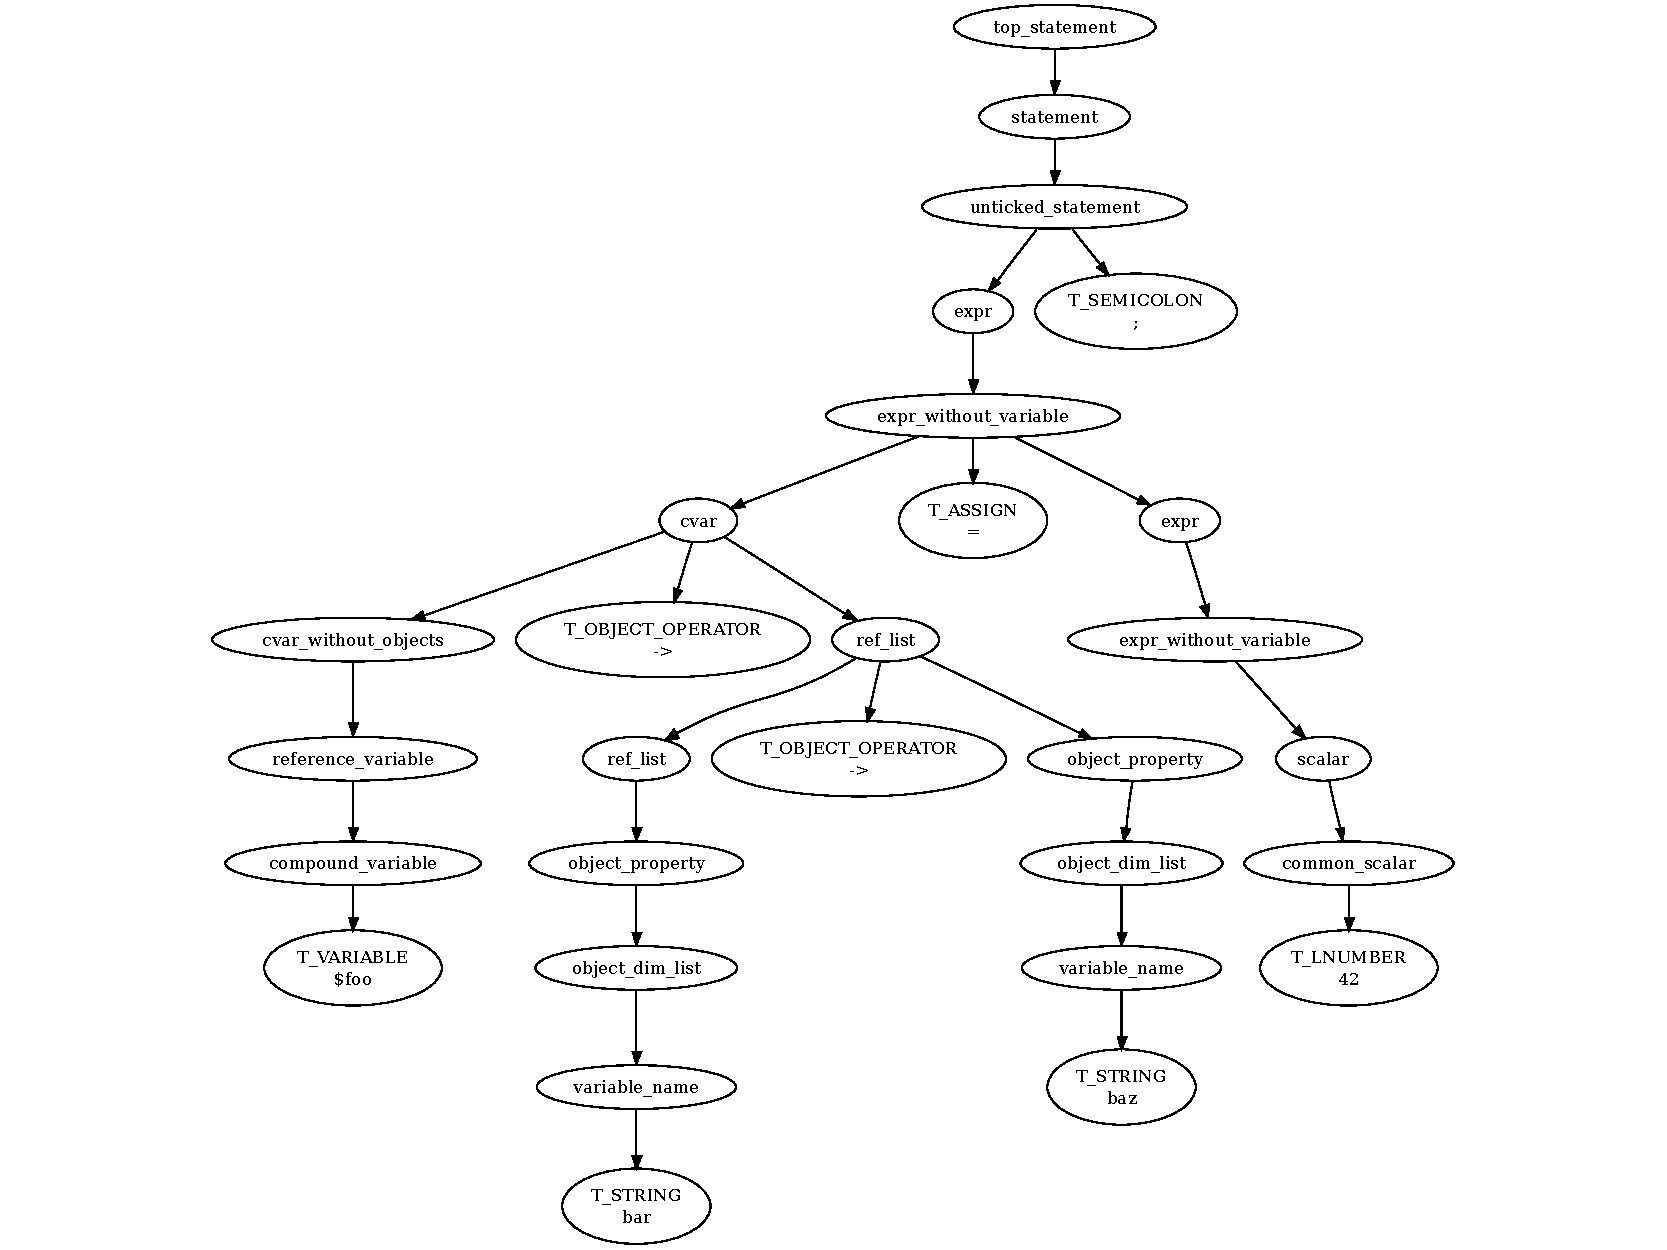
\includegraphics[scale=0.6]{images/multi-level-field-access-left}
   \caption{The PHP parse subtree of \texttt{\$foo->bar->baz = 42;}.}
   \label{fig:multi-level-field-access-left}
  \end{center}
\end{figure}

\begin{figure}[htb]
  \begin{center}
    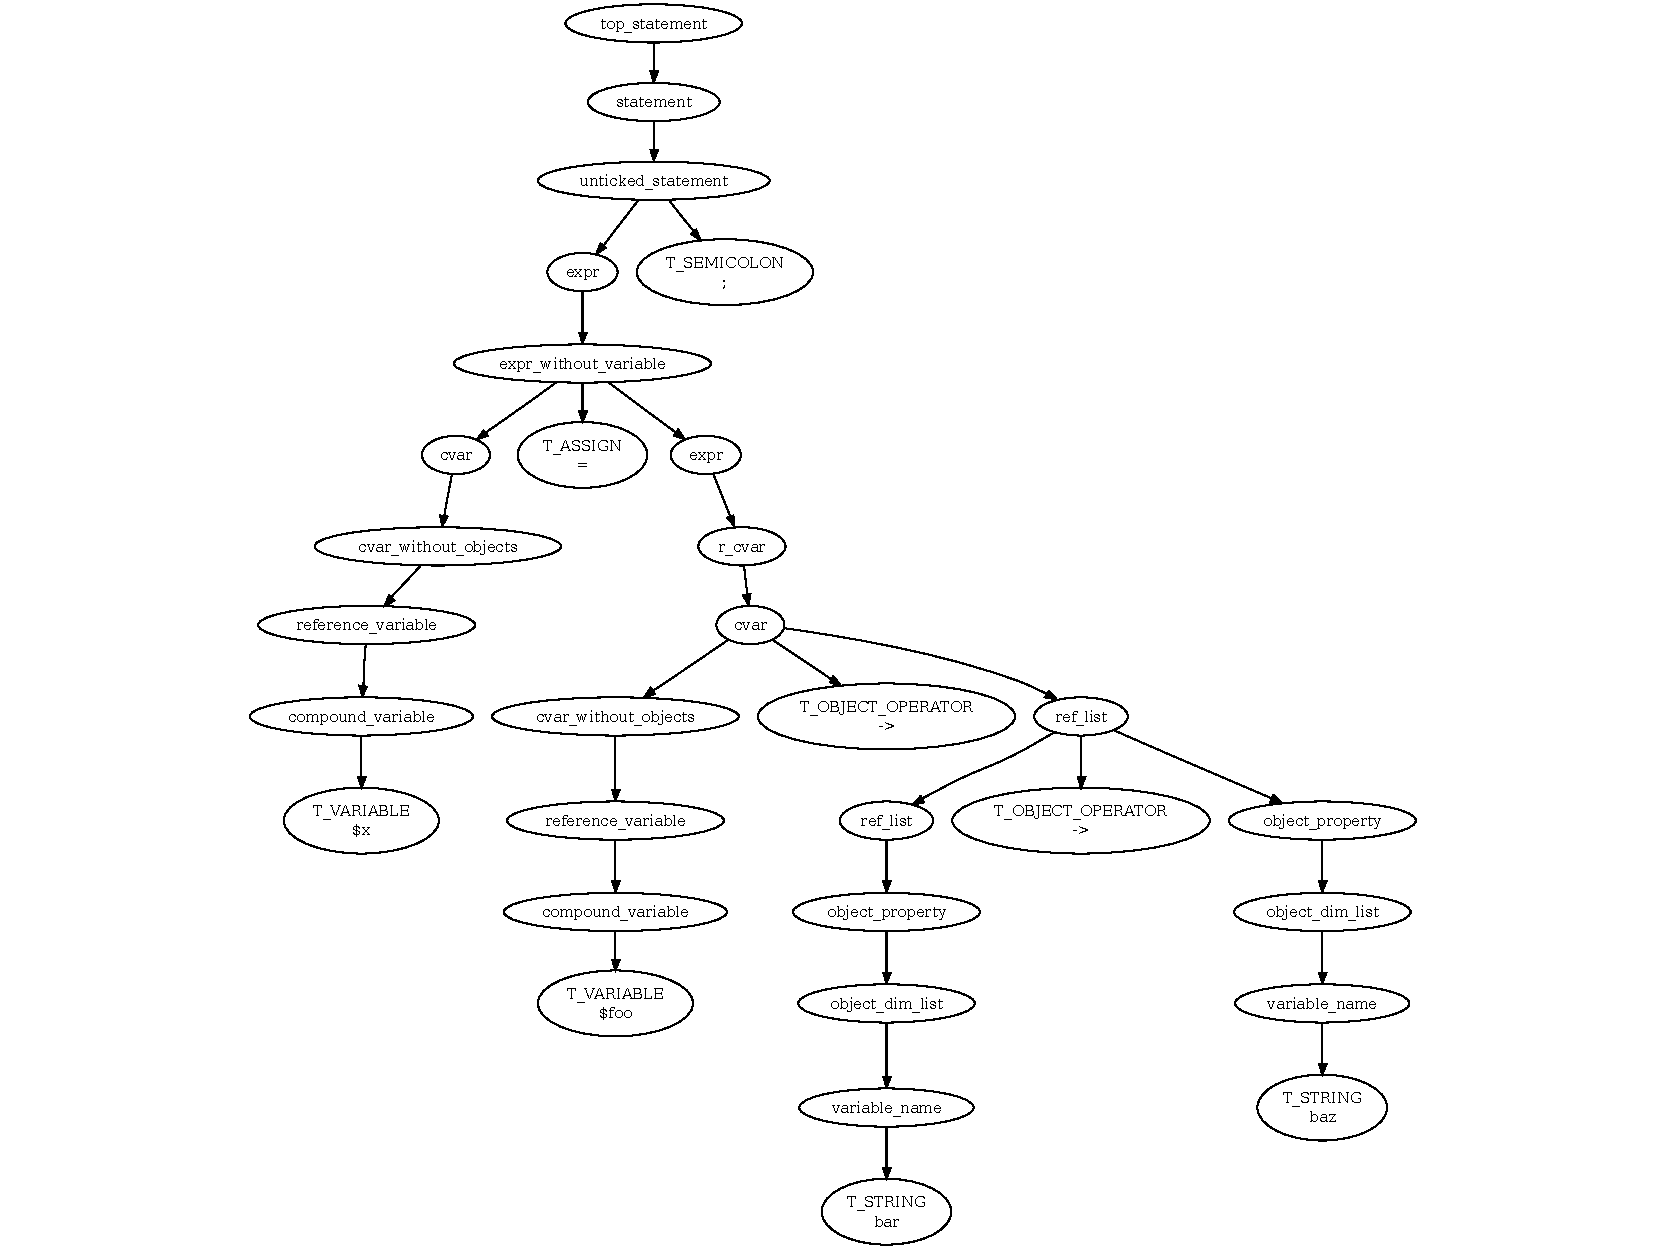
\includegraphics[scale=0.6]{images/multi-level-field-access-right}
   \caption{The PHP parse subtree of \texttt{\$x = \$foo->bar->baz;}.}
   \label{fig:multi-level-field-access-right}
  \end{center}
\end{figure}

\begin{figure}[htb]
  \begin{center}
    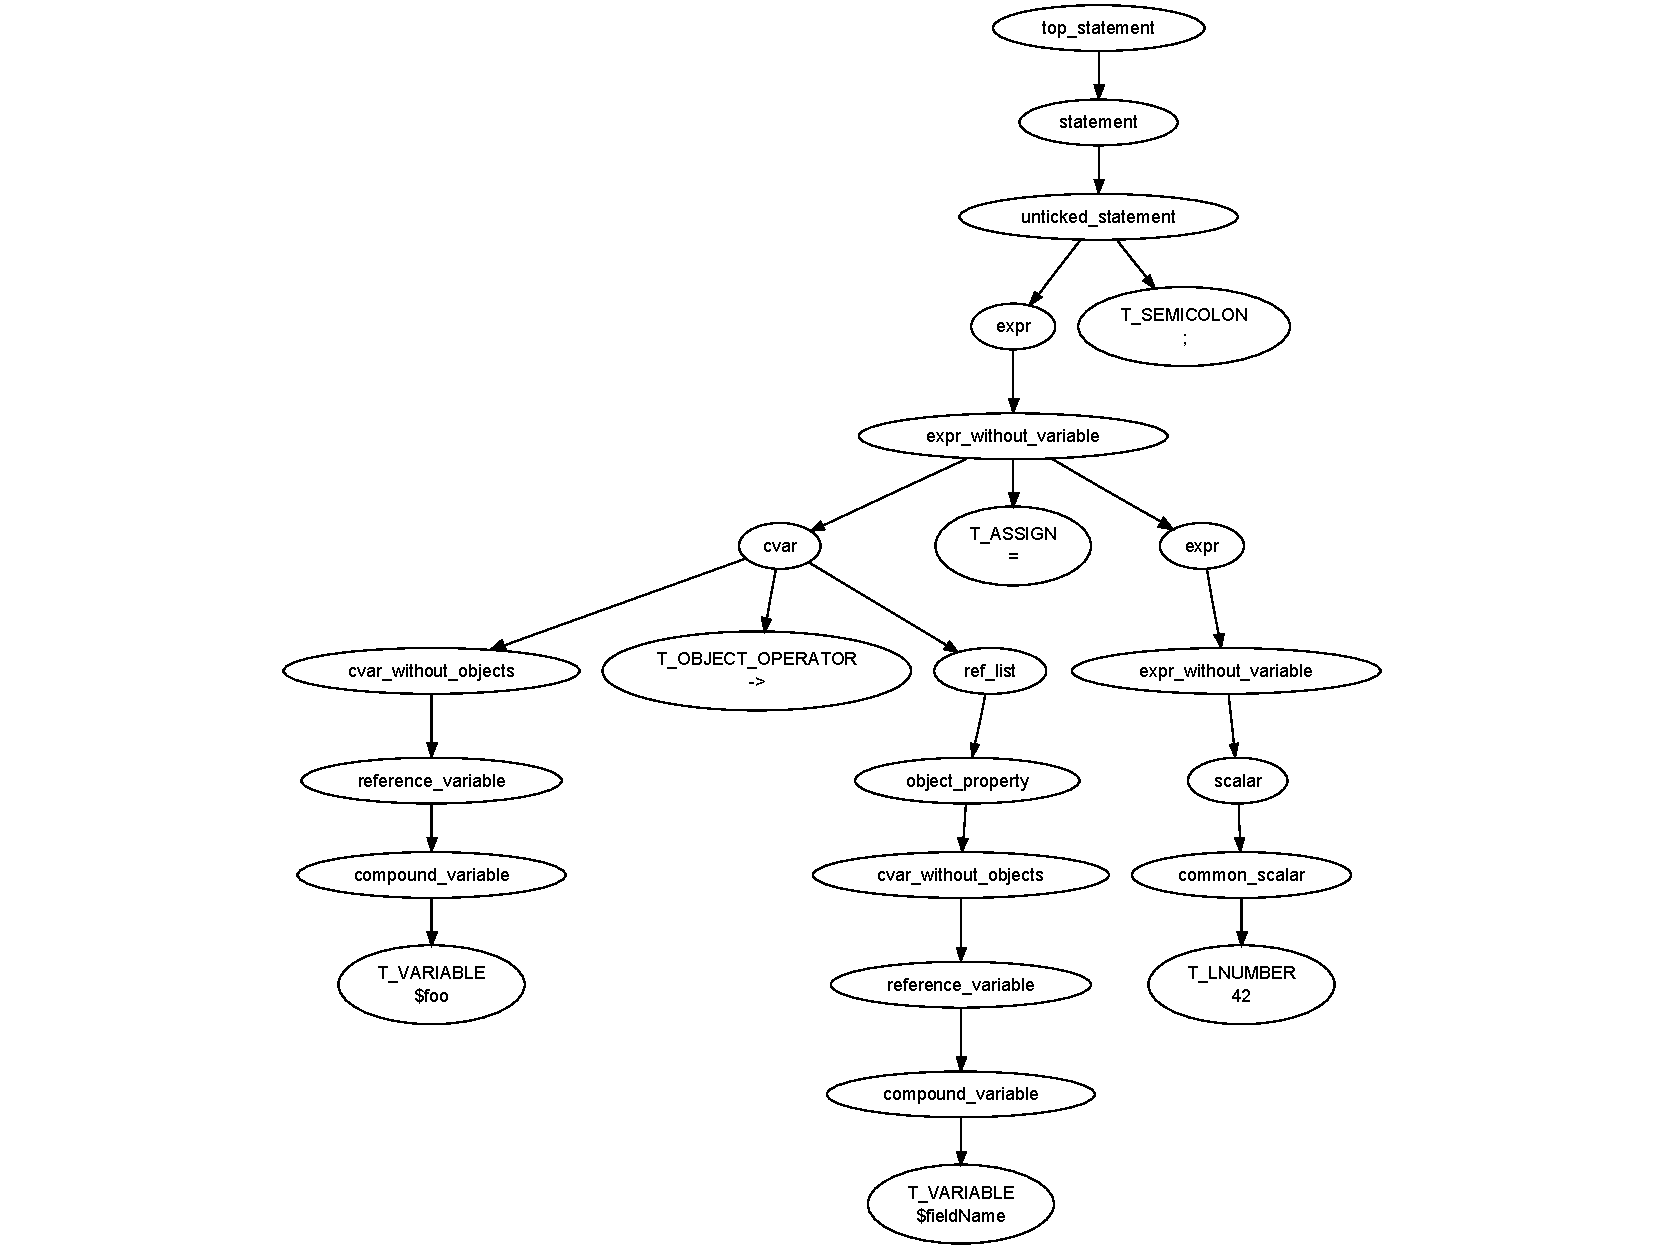
\includegraphics[scale=0.6]{images/variable-field-access-left}
   \caption{The PHP parse subtree of \texttt{\$foo->\$fieldName = 42;}.}
   \label{fig:variable-field-access-left}
  \end{center}
\end{figure}

\begin{figure}[htb]
  \begin{center}
    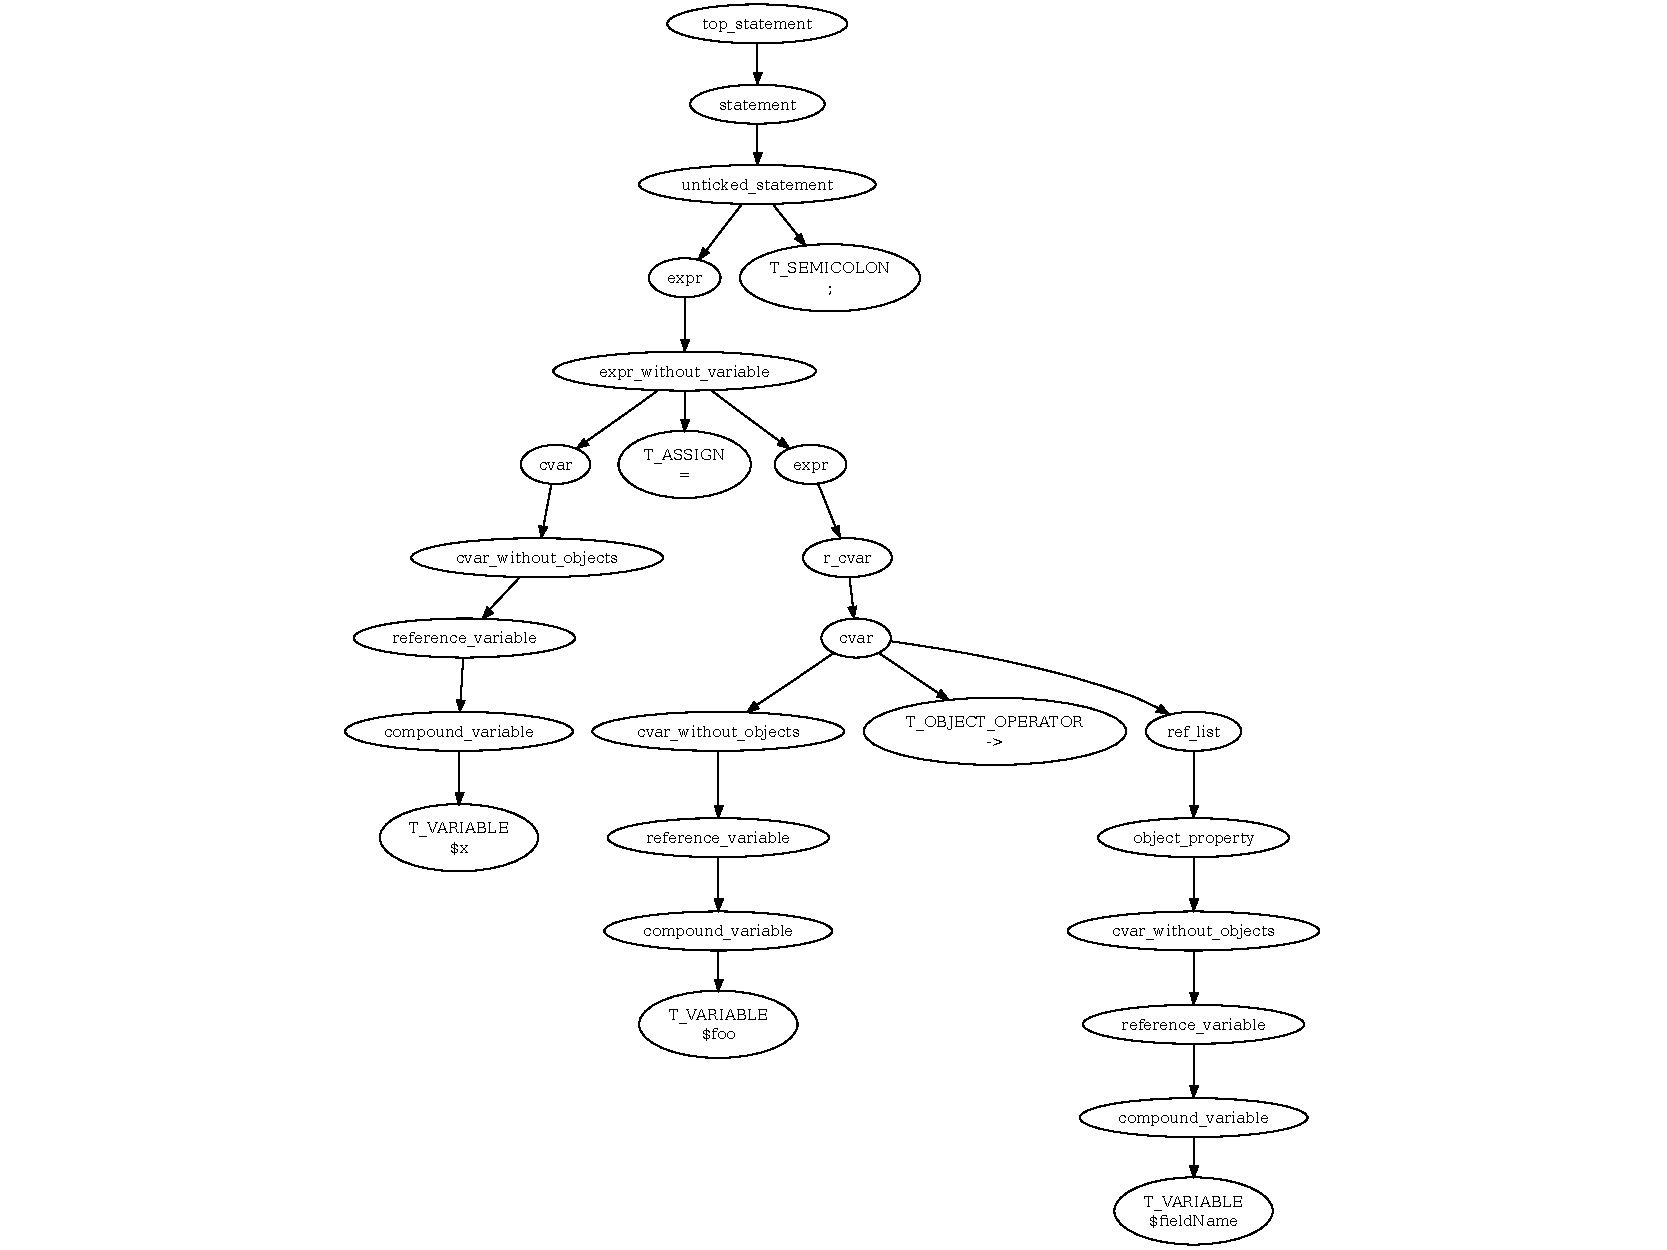
\includegraphics[scale=0.7]{images/variable-field-access-right}
   \caption{The PHP parse subtree of \texttt{\$x = \$foo->\$fieldName;}.}
   \label{fig:variable-field-access-right}
  \end{center}
\end{figure}

As Pixy currently does not model the---relative rare---case of variable variables, this approach does not model them either on the field level.

Looking at the big picture, both for left-side and right-side expressions, the TacConverter walks the field access chain to the end, using existing fields in the object's symbol tables or creating new ones as needed. In pseudo-code that expands the code listed above, this approach looks like this:

\begin{textcode}
assign(subTree) {
  leftPlace = getLeftPlaceFromLeftSubtree(subtree);
  rightPlace = expr_without_variable(subTree->rightChild->firstChild);
  createCfgNodeForAssignment(leftPlace, rightPlace);

  variableName = getVariableNameFromLeftSubtree(subtree);
  if (isSimpleVariable(variableName)) {
    addVariableToSymbolTable(variableName, rightPlace);
  }
}

AbstractPlace expr_without_variable(subtree) {
  // Extract children from subtree here.
  if (secondChild == T_ASSIGN) {
    assign(subtree);
   return null;
  }

  if (firstChild == T_NEW) {
    return new ObjectVariable();
  }
  // More existing code for processing variables and literals.
}

AbstractPlace getLeftPlaceFromLeftSubtree(subtree) {
  fieldChain = createFieldChainFromSubtree(subtree);
  leftmostVariable = retrieveOrCreateVariableFromSymbolTable(fieldChain[0]);
  if (fieldChain->length == 1) {
    // simple variable
    return leftmostVariable;
  }

  subtreeAfterFirstArrow = getSubtreeAfterFirstArrow(subtree);
  leftmostVariable->add
}

/**
 * @return e.g., ["$foo", "bar", "baz"] for $foo->bar->baz
 */
String[] createFieldChainFromSubtree(subtree) {
  ...
}

// Note: To be expanded on Monday.

\end{textcode}
